% !TeX root =../../main.tex

\chapter{Introduction} \label{ch:introduction}

Software systems usually suffer from various kinds of vulnerabilities and weakness. These vulnerabilities can cause huge catastrophes from financial property loss to massive personnel casualty. For example, \emph{Heartbleed} is a critical vulnerability in the widely used OpenSSL cryptographic software library which can compromise the integrity of communications across the entire Web. Due to the  worse still, it is reported that this may also affect the internal networks of enterprise in the coming years due to the fact that most enterprises do not have a good handle on the SSL encrypted services. 


\section{Motivations and Challenges}

\section{Main Work}

\section{Contributions of the Thesis}

\begin{figure}[ht]
	\begin{center}
		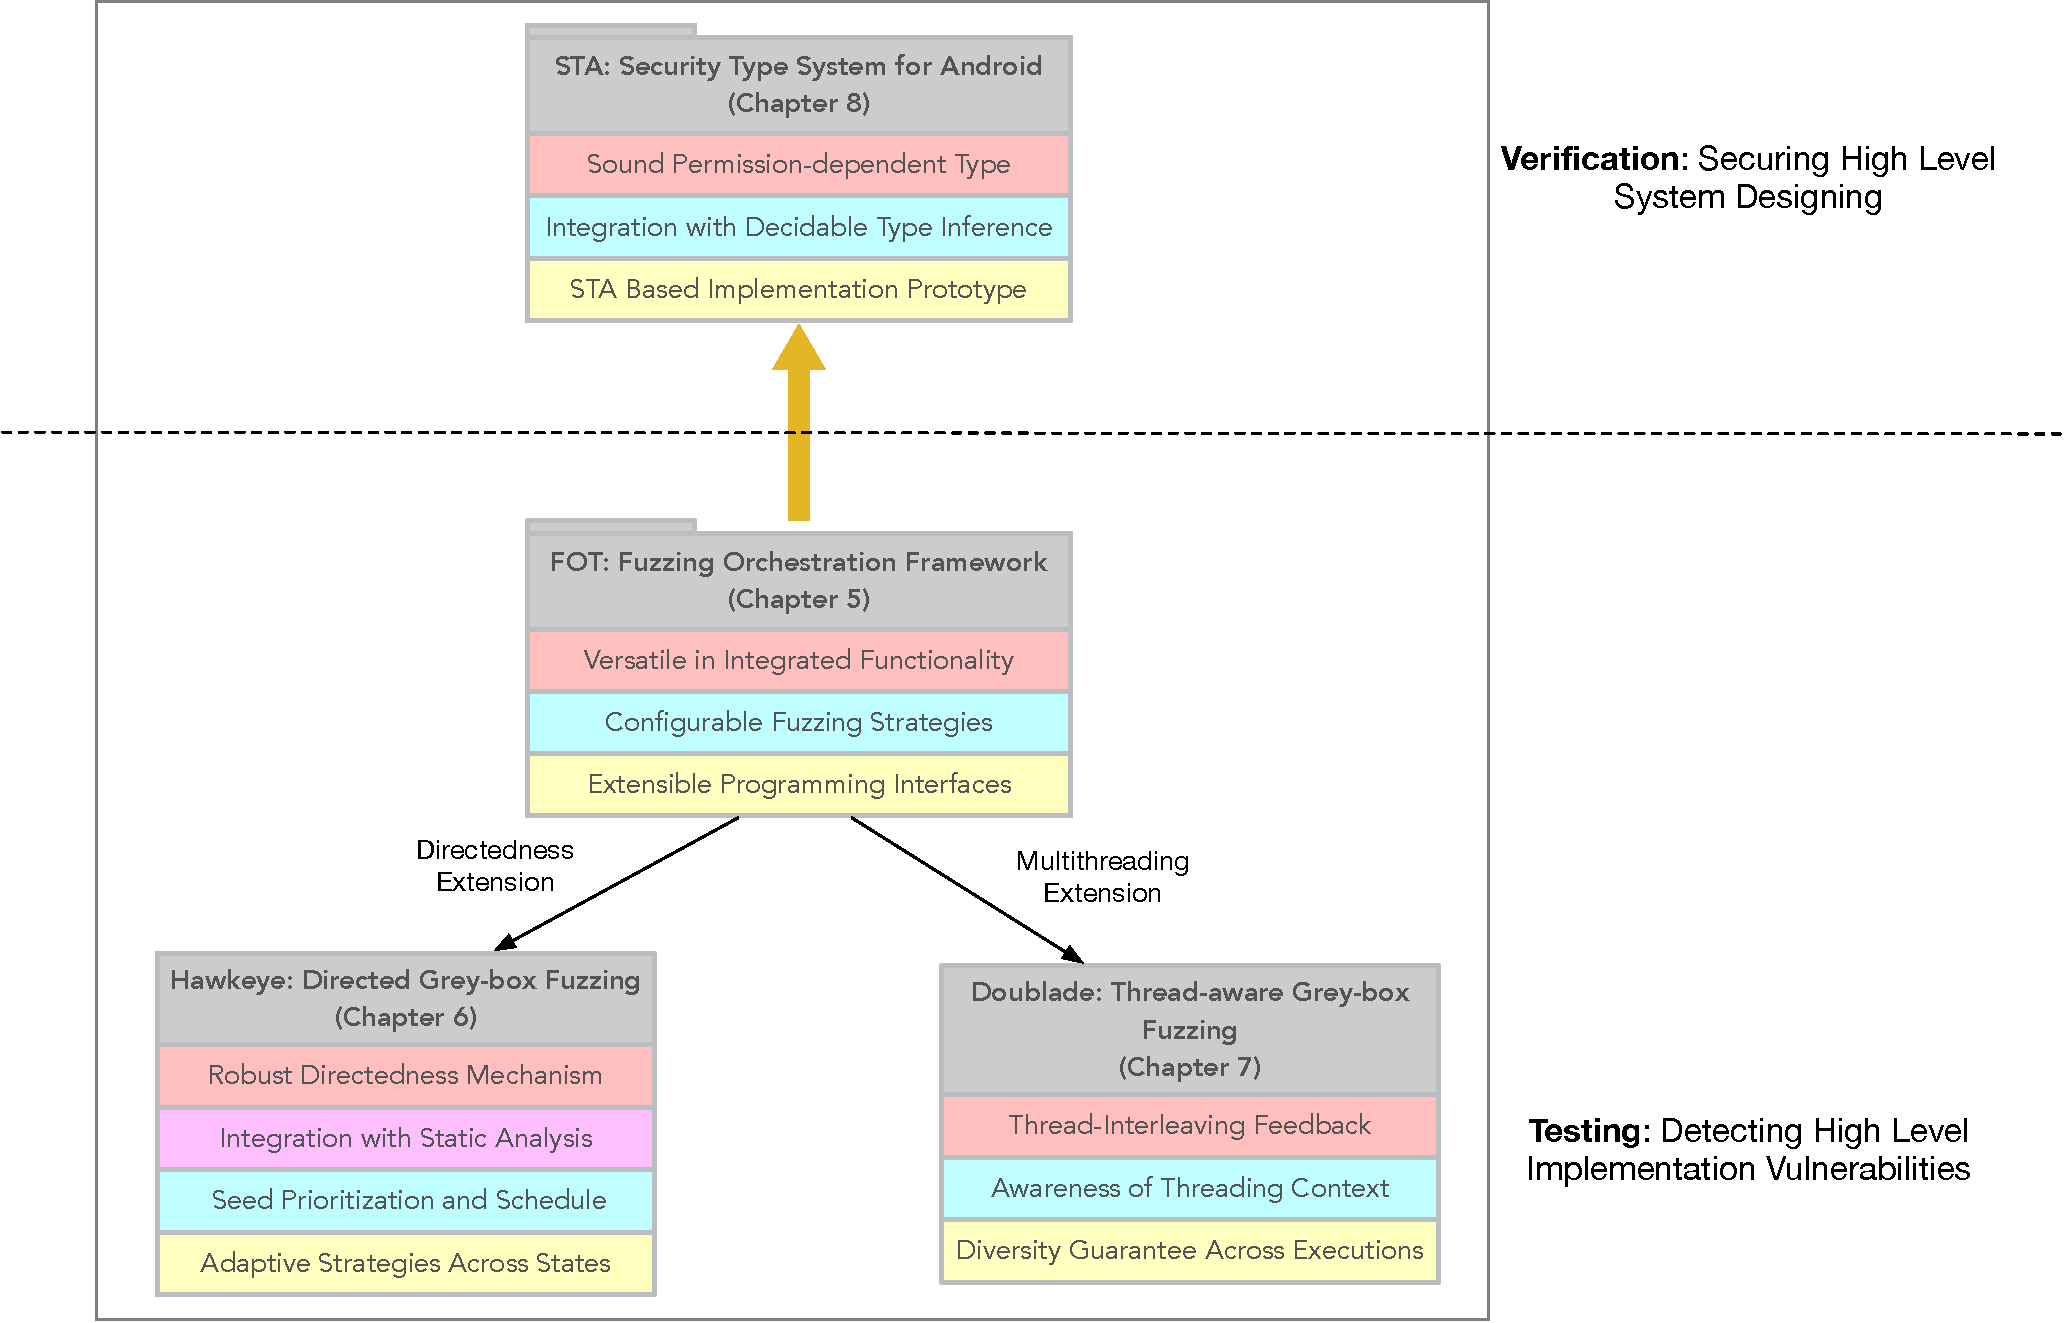
\includegraphics[width=0.98\textwidth]{res/contributions}
		\caption{Contributions of the Thesis and their Relations}
		\label{fig:works}
	\end{center}
\end{figure}


\section{List of Materials Related to the Thesis}

\section{Outline of the Thesis}

The rest of this thesis is organized as follows.

Chapter~\ref{ch:fot} describes the recent progress of fuzzing and several aspects of challenges, and introduces our grey-box fuzzing framework, \FOT, which aims to solve these issues. Chapter~\ref{ch:dfot} explains our directed grey-box fuzzer \dFOT built on top of \FOT; \dFOT is our attempt to guide the fuzzing process to specific program targets. Chapter~\ref{ch:mtfuzz} describes \mtfuzz based on \FOT, which aims to enhance the effectiveness of fuzzing on multithreaded programs. Chapter~\ref{ch:sta} describes our attempt to secure software systems based on verification, which applies a permission-dependent type system to enforce the non-interference property that prevents the information leakage in an Android-like system. Chapter~\ref{ch:discuss} discusses my reflection on the testing and verification based techniques. Chapter~\ref{ch:conclusion} concludes this thesis and describes the possible future work.